\documentclass[e4_tp2_main.tex]{subfiles}
\begin{document}
\newgeometry{top=2.5cm, bottom=2.0cm, left=2.25cm, right=2.25cm}

\section{Modulación PWM y realimentación}

\subsection{Amplificador de error}

\subsubsection*{a) Valores de $R2$ y $R3$ si $V_o=25 VDC$}

Como $V_{FB}$ es el divisor de tensi\'on de $V_o$ y se busca cumplir $V_{FB}=V_{REF}$, se obtiene:

\begin{equation}
V_{FB}=V_{REF}= V_o \cdot \frac{R_3}{R_2+R_3}
\label{ec1.1.a1}
\end{equation}


Depejando de la ecuaci\'on \eqref{ec1.1.a1} y suponiendo que $R_3=10k \Omega $, obtenemos:

\begin{equation}
R_2=R_3 \cdot \left( \frac{V_o}{V_{REF}} - 1 \right)=90k \Omega \label{ec1.1.a2}
\end{equation}

\subsubsection*{b) Transferencia  $\frac{ \widetilde{v_c}(s)}{\widetilde{v_o}(s)}$ para pequeñas variaciones} 

La transferencia a pequeñas variaciones del amplificador de error se obtiene analizando el inversor con $Z_1=R_2$ y $Z_2=R_6 + \frac{1}{sC}$. Esto se debe a que a pequeñas variaciones, tanto la fuente de tensi\'on V2 como la funete de corriente I1 se pasivan.

\begin{equation}
\frac{\widetilde{v_c}(s)}{\widetilde{v_o}(s)}=-\frac{R_6 + \frac{1}{s \cdot C_2} }{R_2} = - \frac{R_6}{R_2} \cdot \frac{s+\frac{1}{C_2 \cdot R_6}}{s} \label{ec1.1.b}
\end{equation}

\subsubsection*{c) Amplificador de error como bloque de un sistema LTI. Ganancia, Polos y Ceros}

Reemplazando los valores num\'ericos de la consigna en ecuaci\'on \eqref{ec1.1.b}, el diagrama en bloque resulta: 

\begin{center}
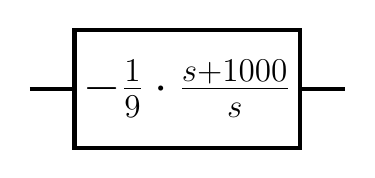
\begin{tikzpicture}[
squarednode/.style={rectangle, draw=black, fill=white!5, ultra thick, minimum size=15mm},
]
\draw[ultra thick] (-2,0) -- (2,0);
\node[squarednode]      (maintopic) {\LARGE {$-\frac{1}{9} \cdot \frac{s+1000}{s}$}};
\end{tikzpicture}
\end{center}


El amplificador de error cuenta con una ganacia $G_{amp}=\frac{1}{9}$, un polo en $s=-1000$ y un cero en el origen.


\subsubsection*{d) Conjunto fuente de corriente I1 y R7}


\subsection{Modulaci\'on PWM}

\subsubsection*{a) Caracter\'isticas de la se\~nal triangular}
\subsubsection*{b) Duty cycle m\'aximo}
\subsubsection*{c) Modulador PWM como bloque de un sistema LTI.}



\subsection{Convertidor DC/DC}
\subsubsection*{a) Funci\'on transferencia del convertidor}

Considerando el diodo y el MOS como ideales, comenzamos analizando el espacio de estados. 

Durante el tiempo que la llave se encuentra cerrada (SW=ON) obtenemos:

\begin{equation}
\underbrace{
\begin{bmatrix}
\dot{i_{L_1}} \vspace{0.2cm} \\
\dot{V_{C_1}} 
\end{bmatrix}
}_{\dot{X}}
=
\underbrace{
\begin{bmatrix}
{0} & {0} \vspace{0.2cm}\\
{0} & {-\frac{1}{R_L \cdot C_1}} 
\end{bmatrix}
}_{A_{on}}
\underbrace{
\begin{bmatrix}
{i_{L_1}} \vspace{0.2cm}\\
{V_{C_1}} 
\end{bmatrix}
}_{X}
+
\underbrace{
\begin{bmatrix}
{\frac{1}{L_1}} \vspace{0.2cm}\\
{0} 
\end{bmatrix}
}_{B_{on}}
V_1
\end{equation}


\begin{equation}
V_o =
\underbrace{
\begin{bmatrix}
{0} & {1} 
\end{bmatrix}
}_{C_{on}}
\begin{bmatrix}
{i_{L_1}} \\
{V_{C_1}} 
\end{bmatrix}
\end{equation}

Por otro lado, durante el tiempo que la llave se encuentra abierta (SW=OFF), se obtiene que: 

\begin{equation}
A_{off} = 
\begin{bmatrix}
{0} & {- \frac{1}{L_1}} \vspace{0.3cm}\\ 
{\frac{1}{C}} & {-\frac{1}{R_L \cdot C_1}}
\end{bmatrix}  
\hspace{2cm} B_{off}=B_{on}  
\hspace{2cm} C_{off} = C_{on}
\end{equation}


A continucaci\'on se calcula el promedio ponderado de las matrices de estado:

\begin{equation}
\overline{A} = A_{on} \cdot d + A_{off} \cdot (1-d) \hspace{2cm} \overline{A}=A_{on} = A_{off}  \hspace{2cm} \overline{B}=B_{on} = B_{off}  
\end{equation}

Finalmente, utilizando la ecuaci\'on provista por la c\'atedra en la clase de Transferencias y reemplazando los valores obtenidos anteriormente obtenemos la transferencia deseada. 

\begin{equation}
\frac{ \widetilde{v_o}(s)}{\widetilde{d}(s)}= \overline{C} \cdot (s \cdot I - \overline{A})^{-1} \left[ (A_{on} - A_{off})X(s) + (B_{on} - B_{off}) V_1 \right] +(C_{on} - C_{off})X(s) 
\label{ec1.3}
\end{equation}

Donde X(s) es el vector en estado estacionario:

\begin{equation}
X(s)= 
\begin{bmatrix}
{i_{L_1}} \\
{V_{C_1}} 
\end{bmatrix}
=
\begin{bmatrix}
{\frac{I_o}{1-d}} \vspace{0.3cm} \\
{\frac{V_1}{1-d}} 
\end{bmatrix}
=
\begin{bmatrix}
{\frac{V_1}{R_L(1-d)^2}} \vspace{0.3cm} \\
{\frac{V_1}{1-d}} 
\end{bmatrix}
\end{equation}

\begin{equation}
\frac{ \widetilde{v_o}(s)}{\widetilde{d}(s)}= 
\label{ec1.3}
\end{equation}

% Cuales son las Singularidades del sistema?
\subsubsection*{b) Valor real del Duty cycle}

%Por que es diferente del teorico?
\subsubsection*{c) Tiempos de establecimiento ante los cambios de carga }
\subsubsection*{d) Tiempos de establecimiento con $R_6=22k\Omega$ y $R_6=1k\Omega$}



\end{document}